\documentclass{article}
\usepackage{tikz}
\usepackage{darkmode}
\usepackage{amsmath}
\usepackage{colonequals}
\sloppy
\newcommand*{\logeq}{\ratio\Leftrightarrow}
\enabledarkmode
\author{Pierson}
\begin{document}
\title{Calc III Notes}

\maketitle

\section{Multivariable calc goals}
\begin{list}{-}{}
    \item vectors and geometry of R''
    \item functions of serval variables diff and int
    \item higher dimensional versions of FTC
    \item fund them for line integrals
    \item greens them
    \item stokes them
    \item divergence them
\end{list}

\setcounter{section}{11}
\section{Chapter 12: vectors and geo of space}
\subsection{}
    \begin{list}{-}{}
    \item \[R = line\] dist(x,y) = $ |y - x | $
    \item \[R^2 = Plane\] Orders pairs of (x,y) of real numbers
    \item \[R^3 = space\] ordered triples of (x,y,z) of real numbers
    \end{list}

right-hand rule: point fingers toward pos x-axis and curl towards pos y-axis, thumb should point to positive z\\


$R^n$ = n-tuples $(x_1, x_2, ... x_n)$ n-dim space\\

Distance D from (0,0) to (x,y)
\[D^2 = x^2 +y^2\]

Distance D from (0,0,0) to (x,y,z)
\[ D = \sqrt{x^2+yy^2+z^2}\] 

Sphere with center $X_0, Y_0, Z_0$ and radius R has equation:

\[ (X-X_0)^2 + (y-y_0)^2 + (z-z_0)^2 = r^2 \] 

Find equation of the set of points equidistant from the points a1,4,2, and b 3,3,3

\[AX = \sqrt{(x-1)^2 + (y-4)^2 + (z-2) ^2} \] 
\[ BX = \sqrt{(x-3)^2 + (y-3)^2 + (z-3) ^2} \]

set AX = BX

Result is a \textbf{plane}

\subsection{vectors and geo of space}
scaler = magnitude $\leq 0$ \\
vector = magnitude + direction \\

$\vec{u} = <5,3>$, $\vec{u} =5 \hat{i} +3\hat{j}$ \\

\begin{center}
    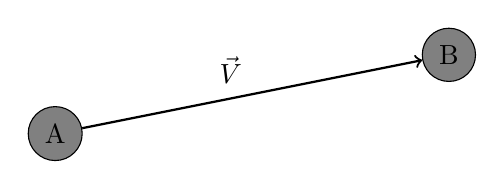
\begin{tikzpicture}
    \node[draw, circle, fill=gray] at (0, 0) (A) {A};
    \node[draw, circle, fill=gray] at (5, 1) (B) {B};
    \draw [thick, ->] (A) -- (B) node[midway, above left] {$\vec{V}$};
    \end{tikzpicture} 
    \linebreak
    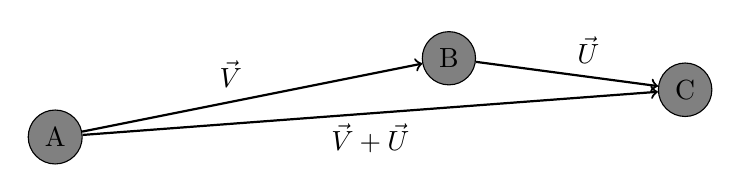
\begin{tikzpicture}
    \node[draw, circle, fill=gray] at (0, 0) (A) {A};
    \node[draw, circle, fill=gray] at (5, 1) (B) {B};
    \node[draw, circle, fill=gray] at (8, .6) (C) {C};
    \draw [thick, ->] (A) -- (B) node[midway,above left] {$\vec{V}$};
    \draw [thick, ->] (B) -- (C) node[midway,above right] {$\vec{U}$}; 
    \draw [thick, ->] (A) -- (C) node[midway,below] {$\vec{V} + \vec{U}$};
    \end{tikzpicture}
\end{center}


\subsubsection{Scaler multiple}

\begin{tikzpicture}
\node at (0, 0) {};
\node at (5, 1) {};
\node[] at (-5, -1) (D) {};
\node[] at (10, 2) (C) {};
\draw [thick, ->] (A) -- (B) node[midway, above left] {$\vec{V}$};
\draw [thick, ->] (A) -- (C) node[midway, above left] {$2\vec{V}$};

\draw [thick, ->] (A) -- (D) node[midway, above left] {$-\vec{V}$};


\end{tikzpicture}

Changes the length of the vectors, ie, stretches them in a direction. 

Length of k$\vec{v} =|K| * |V|$ 

direction of $k\vec{V} = same as \vec{V} if k > 0$

real numbers work like scaling factors \\

Points = (a,b)

Vector = $<a,b>$

\subsubsection{\textbf{Vectors in $R^3$}}

Extra cords for points and extra comps for vectors

point = (a,b,c)

vector = $<a,b,c>$

\[ if \vec{V} = \vec{P_1P_2}, then |\vec{V}| = \sqrt{(x_2 - x_1)^2 + (y_2 - y_1)^2 + (z_2 - z_1)^2}\]
\\
$P(4, -1, -3) \\
Q(8, 0 , -5) \\
R (0, -2, -1)$
\\
\\
$\vec{PQ} = <8-4, 0 --1, -5  --3>$

\[\vec{u} = <3, 1, 3>\]
\[\vec{v} = <1,3,7>\]
\[\vec{v} +\vec{v} = <3+1, 1+3, 3+7>\]

\[5 * \vec{v} = <1*5, 3*5, 7*5>\]

\subsubsection{notation}

\[V_n\] set of all n-dim vectors $<V_1, V_2, ..., V_n>$

$V_3$ set of all vectors $<v_1, v_2, v_3>$
\\ 
$\hat{i} = <1, 0, 0>$ \\
$\hat{j} = <0, 1, 0>$ \\
$\hat{k} = <0, 0, 1>$ \\

unit vector = vector of length 1

$\hat{i}, \hat{j}, \hat{k}$ are unit vectors

find the unit vector that has the same direction as $\vec{b} = 4\hat{i} -2\hat{j} +3\hat{k}$

\[\sqrt{4^2 (-2)^2 + 3^2}\]
\[\sqrt{16 +4 + 9 }\]
\[\sqrt{29}\]
\[\frac{\vec{b}}{|\vec{b}|} = \frac{1}{\sqrt{29}}(4\hat{i} -2\hat{j} +3\hat{k})\] \\

\subsubsection{dot product}
dot product $\rightarrow$  2 vectors $\rightarrow$ 1 scaler \\
cross product $\rightarrow$  2 vectors $\rightarrow$ 1 vector \\

\[\vec{a} \cdot \vec{b} = a_1b_1+a_2b_2+a_3b_3\]

\textbf{Properties}
\[\vec{a} \cdot \vec{a} = \vec{a}^2\]

if $\theta$ is the angle between the vectors $\vec{a}$ and $\vec{b}$, then $\vec{a} \cdot \vec{b} =|\vec{a}||\vec{b}|\cos(\theta)$ \\

follows from the law of cosines \\

$\vec{a}$ and $\vec{b}$ are orthogonal (or perp) if te angle between them is $\theta=\frac{\pi}{2}$ \\

the zero vector $\vec{0}$ is considered orthogonal to all vectors \\

$\vec{a} \cdot \vec{b} = 0 <=> \vec{a} \perp \vec{b}$, orthogonal, form 90$\deg$ angle

\begin{center}
accute
\[ \vec{a} \cdot \vec{b} > 0 \]
obtuse
\[ \vec{a} \cdot \vec{b} > 0 \]
\end{center}

find angle $\theta$ between $a =<1,1,5>$ and $b=<0,3,4>$

\begin{center}
    
    a = $\sqrt{1^2+ 1^2+ 5^2}$
    
    b = $\sqrt{0^2 +3^2+ 4^2}$

    $\cos\theta = \frac{\vec{a}\vec{b}}{|\vec{a}|\vec{b}|}$

    $\cos\theta = \frac{23}{3\sqrt{3} \times 5}$

    $\theta = \arccos(\frac{23}{15\sqrt{3}})$
\end{center}

\subsection{Projections}

$proj_{\vec{a}}(\vec{b}) =$ vector projection of $\vec{b}$ onto $\vec{a}$ \\
Vector           = A scaler-multiple of $\vec{a}$\\


$comp_{\vec{a}}(\vec{a}) =$ Scaler projection of $\vec{b}$ onto $\vec{a}$ \\
Scaler           =  Signed magnitude of the vector projection \\
                 = $|\vec{b} cos\theta|$\\


\textbf{dot product}

\begin{list}{-}{}
\item valid in any dim
\item result is a scaler
\item application:work
\end{list}

\textbf{cross product}
\begin{list}{-}{}
\item valid in only $r^3$
\item result is a vector 
\item application: torque
\end{list}

$\hat{i} \times \hat{j} = \hat{k}$

\[\vec{a} \times \vec{b} = -\vec{b} \times \vec{a}\]


\subsection{}

\subsection{Equations of lines and planes}

line segment from $\vec{r_{0}}$ to $\vec{r_{1}}$

\[\vec{r} = \vec{_{0}} +t(\vec{r_{1}} -\vec{r_{0}}), 0\leq t \leq 1\]

\begin{center}
    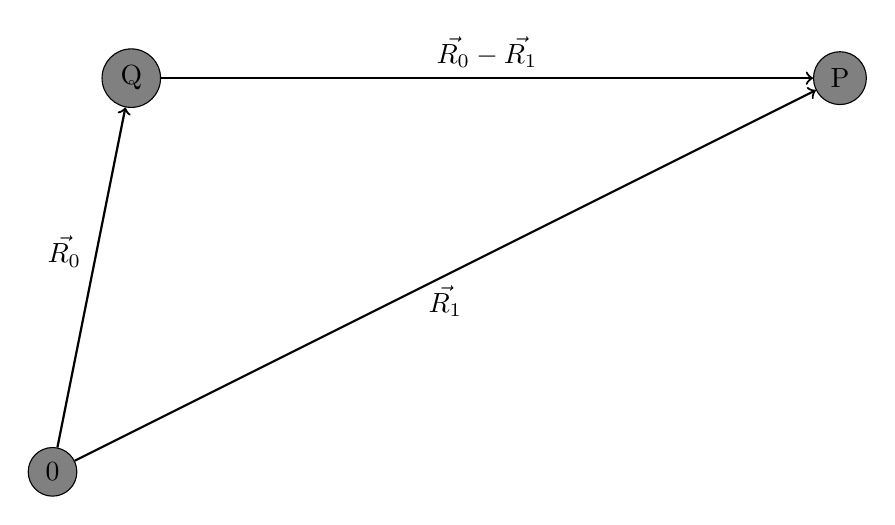
\begin{tikzpicture}
        \node[draw, circle, fill=gray] at (0, 0) (0) {0};
        \node[draw, circle, fill=gray] at (1, 5) (Q) {Q};
        \node[draw, circle, fill=gray] at (10, 5) (P) {P};
        \draw [thick, ->] (0) -- (Q) node[midway,above left] {$\vec{R_{0}}$};
        \draw [thick, ->] (Q) -- (P) node[midway,above] {$\vec{R_0} - \vec{R_1}$}; 
        \draw [thick, ->] (0) -- (P) node[midway,below] {$\vec{R_1}$};
    \end{tikzpicture}
\end{center}
EX: Find parametric eq for the line seg from P(1,-3,5) to Q(4,-7,2)

\subsubsection{Planes in $R^3$}
How to specify plane?
\begin{list}{-}{}
\item specify a point $P_0 \approx (x_0, y_0, z_0) on plane$
\item and a normal vector $\vec{n} = <a,b,c> \neq \vec{0}$ which is perp to the plane
\end{list}

Then P (x,y,z) is in plane $\logeq \vec{n} $ and $ \vec{p_0}\vec{p}$ are orth 
\[\vec{n} \cdot \vec{p_0P} = 0\]
\begin{center}
    \textbf{\large eqn of a plane} \\
    $a(x-x_0) + b (y-y_0) + c (z - z_0) = 0$ \\
    or \\
    $ax+by+cz + d =0$, where $d = -(ax_0+by_0+cz_0)$
\end{center}

Ex. Find an eqn of the plane through points 
\[P_1(0,1,4)\]
\[P_2(2,4,1)\]
\[P_3(3,-1,5)\]
\[\vec{V} = \vec{P_1P_2} = <2,3,-3> = P_2 -P-1 \]
\[\vec{W} = \vec{P_1P_3} = <3,-2,1> = P_3 -P-1 \]
\[\vec{N} = \vec{V} \times\vec{W} = 
\begin{bmatrix}
    \hat{i} & \hat{j} & \hat{k} \\
    2 & 3 & -3 \\
    3 & -2 & 1 \\
\end{bmatrix} 
= -3\hat{i}-11\hat{j}-13\hat{k} \] \\

\begin{center}
    PLANE:   $P_1(0,1,4), \vec{n} = <-3,-11,-13>$
\end{center}
\[-3(x-0) + -11 (y-1) + -13 (z - 1) = 0\]
\[+3(x-0) + 11 (y-1) + 13 (z - 1) = 0\]
\[+3(x) + 11y + 13z -63 = 0\]


\begin{center}
    EX: Find an eqn of a plane that is parallel to the plane $*x-y-3z+3=0$ and goes through the point (5,6,7)
    \[8(x-5) - 1(y-6) -3(z-7) = 0\]
\end{center}
\begin{center}
    Angle between two planes = Angle btween their normal vectors \\
    use $\cos\theta =\frac{\vec{n_1}\cdot\vec{n_2}}{|\vec{n_1}||\vec{n_2}|}$
\end{center}

Sketching a plane\\
3 noncollinear points determine a plane \\
find interactions with x,y,z axes \\
then draw plane between them \\

\subsubsection{Intersections}

ex: line and plane 

\begin{center}
    \noindent \textbf{\large Line=}
\end{center}
\[X =2 -3t\]
\[y=1+4t\]
\[z=-1+2t\]

\begin{center}
    \noindent \textbf{\large Plane = }
\end{center}
\[8x -y -3z+3=0\]

\[8(2+3t) -(1+4t) -3(-1+2t) +3=0\]
\[21+14t=0\]
\[t=-\frac{3}{2}\]
\linebreak
\begin{center}
    \noindent \textbf{\large ex: plane and plane}
\end{center}
\[plane 1 = 8x-y-3z+3 = 0\]
\[plane 2 = -4x+y+2z+5 = 0\]

First method: introduce a parameter. z=t
\[plane 1 = 8x-y-3t+3 = 0\]
\[plane 2 = -4x+y+2t+5 = 0\]
\[P_1+P_2 = 4x -t +8 =0\]
\[x=\frac{1}{4}t-2\]

\[8(\frac{1}{4}t-2)-y-3t+3 = 0\]
\[-t-13=y\]

\[x=2+1/4t\]
\[y-13-t\]
\[z=t\]

\subsubsection{Parametric equations}
\begin{center}
    Uses both a point and a vector. Pretty much a spot where the line starts, and then what direction it is going. 

    When parametrizing you then say it lies along this line at some time $t$, with $-\infty < t < \infty$. 

    For a line through $P_0(x_0, y_0, z_0)$ 


    \[\vec{V} = v_1 \hat{i} + v_2\hat{j} +v_3\hat{k}\]
    \[x = x_0 + tv_1\]
    \[y = y_0 + tv_2\]
    \[z = z_0 + tv_3\] 

\end{center}
\[\]

\section{Chapter 13: vector functions}

\section{Chapter 14: partial derivate}

\section{Chapter 15: multiple integrals}

\section{Chapter 16: vector calculus}

\section{Examples}


\end{document}